Caja Incasur es una empresa líder en el sector financiero, dedicada a ejecutar distintas actividades, entre ellos, una en donde ejecutivos realizan un formulario para registrar sus actividades diarias, con el fin de llevar un control de las mismas. Sin embargo, el proceso actual es mediante un formulario de Google propenso a errores, lo que dificulta la gestión eficiente de la información y el seguimiento de las actividades, además que realizar informes analíticos es muy laborioso.

Como se observa en las figuras \cref{fig:forms1}, \cref{fig:forms2}, \cref{fig:forms3} y \cref{fig:forms4}, el formulario actual de registro de actividades diarias en Caja Incasur consta de varias secciones, cada una con campos específicos para ingresar información relevante sobre las actividades realizadas por los ejecutivos. Este proceso manual no solo es propenso a errores humanos, sino que también dificulta la consolidación y análisis de los datos, lo que puede afectar la toma de decisiones informada y oportuna dentro de la empresa, además que las 2 últimas preguntas en la \cref{fig:forms4} no aplican para todos los usuarios y al no ser dinámico, limita la capacidad de adaptación a los cambios en los requisitos del negocio.

Se propone desarrollar una aplicación móvil en Flutter y otra web con Astro + React que permita a los ejecutivos de Caja Incasur registrar sus actividades diarias de manera más eficiente y para que el gerente o encargado pueda supervisar el progreso respectivamente. La aplicación móvil contará con una interfaz intuitiva y amigable, diseñada para facilitar la entrada de datos y minimizar los errores. Además, en la aplicación móvil se implementarán funcionalidades para generar informes analíticos de manera automática.


\begin{figure}[H]
    \centering
    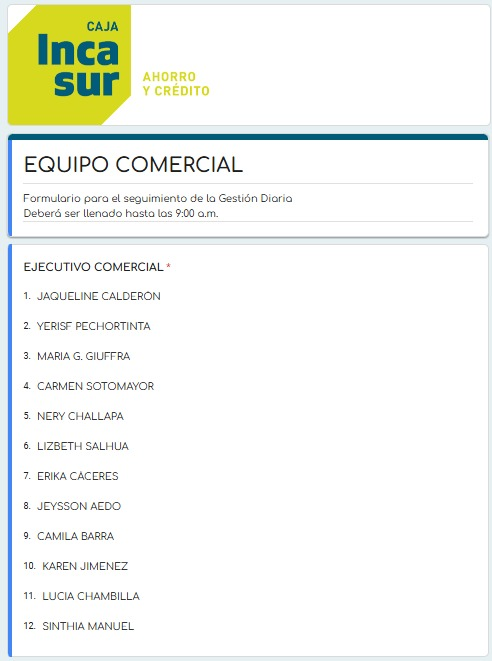
\includegraphics[width=\columnwidth]{media/design/2026-04-27-05-09-53.png}
    \captionof{figure}{Formulario actual de registro de actividades diarias en Caja Incasur parte 1}
    \label{fig:forms1}
\end{figure}

\begin{figure}[H]
    \centering
    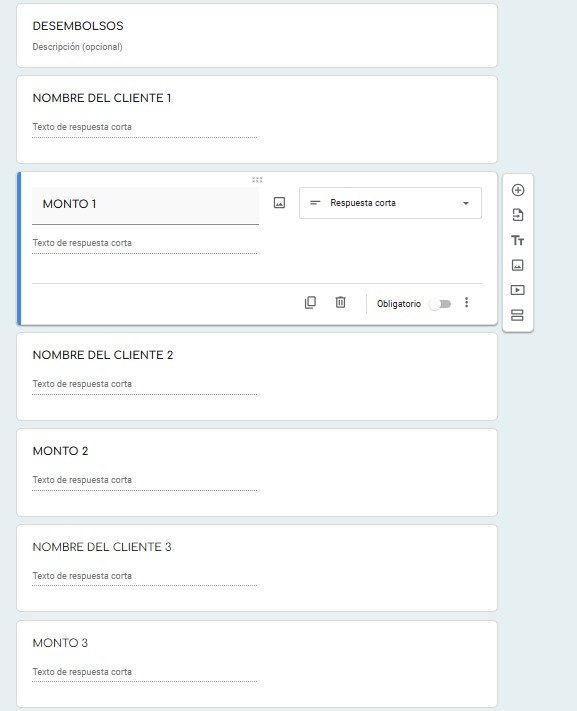
\includegraphics[width=\columnwidth]{media/design/2026-04-27-05-11-33.png}
    \captionof{figure}{Formulario actual de registro de actividades diarias en Caja Incasur parte 2}
    \label{fig:forms2}
\end{figure}


\begin{figure}[H]
    \centering
    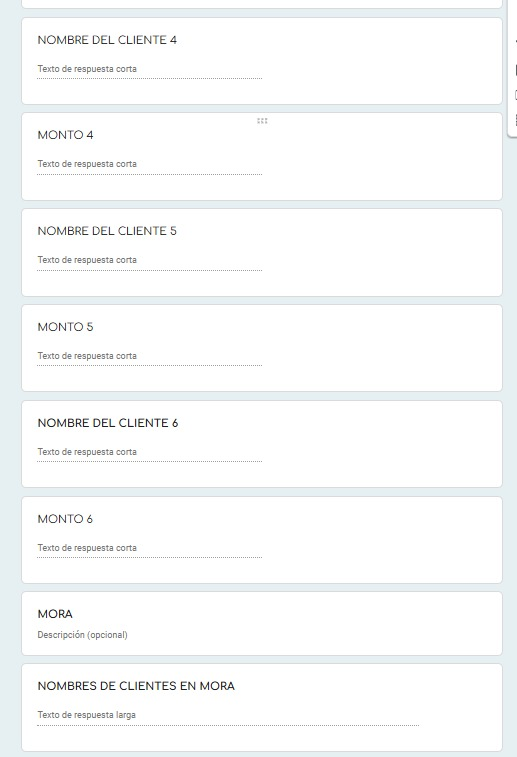
\includegraphics[width=\columnwidth]{media/design/2026-04-27-05-12-27.png}
    \captionof{figure}{Formulario actual de registro de actividades diarias en Caja Incasur parte 3}
    \label{fig:forms3}
\end{figure}


\begin{figure}[H]
    \centering
    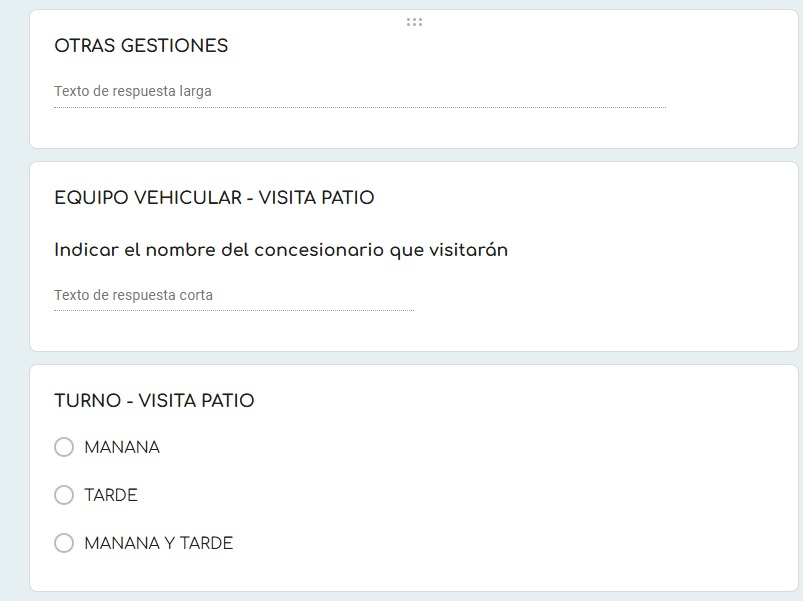
\includegraphics[width=\columnwidth]{media/design/2026-04-27-05-14-06.png}
    \captionof{figure}{Formulario actual de registro de actividades diarias en Caja Incasur parte 4}
    \label{fig:forms4}
\end{figure}

El sistema propuesto tendrá en cuenta los datos mediante la integración del concepto de Ant Colony Optimization (ACO). En esta arquitectura, el flujo de trabajo se modela como un grafo dinámico donde los ejecutivos actúan como agentes ("hormigas") que depositan feromonas digitales en las rutas de éxito comercial. Cada interacción exitosa, desde la prospección hasta el desembolso, refuerza un camino específico, permitiendo que el sistema aprenda colectivamente cuáles son los perfiles de cliente y productos con mayor probabilidad de cierre en tiempo real.


Para el ejecutivo comercial, el sistema automatiza la priorización de su cartera mediante una lista dinámica de llamadas y gestiones. En lugar de seguir un orden cronológico simple, el algoritmo ordena las tareas según la intensidad de la feromona depositada por el enjambre en actividades similares. Esto optimiza el proceso de registro diario, permitiendo al personal de campo enfocar sus esfuerzos en los leads que presentan una mayor "frescura" y probabilidad de conversión, maximizando así la eficiencia operativa de la entidad financiera.

Desde la vertiente administrativa, el sistema elimina la dependencia de reportes manuales y hojas de cálculo estáticas. Mediante un Dashboard de Salud Diaria, el gerente puede supervisar el rendimiento de las distintas líneas de negocio (Vehicular, Pyme, Convenio) a través de la visualización de la densidad de feromonas.

\begin{itemize}
    \item El sistema agrupa automáticamente los montos por línea operativa; una alta actividad se traduce en una "feromona brillante", mientras que la ausencia de registros activa alertas rojas de estancamiento, permitiendo intervenciones correctivas inmediatas antes del cierre mensual.
    \item La herramienta introduce una métrica de envejecimiento de créditos, al rastrear el tiempo transcurrido desde la primera aparición de un cliente en el formulario hasta su desembolso, el ACO detecta cuándo una feromona comienza a "evaporarse" debido a la inactividad. Esto permite al gerente identificar cuellos de botella específicos y predecir con alta precisión el ingreso real de capital, diferenciando los créditos con alta probabilidad de cierre de aquellos que se han estancado en la fase de evaluación.
\end{itemize}